\documentclass[12pt,a4paper]{article}
\usepackage{color}
\usepackage{amsmath}  
\usepackage{amsthm}
\usepackage{amssymb}
\usepackage{amsfonts}
\usepackage{graphicx}  


\begin{document}

\title{Bethe Ansatz Solution of ASEP with Reflecting Boundaries}
\author{Wenwen Huang}
\date{\today}
\maketitle

\section{Single Particle Solution}
\label{sec:single_particle_solution}

To investigate the ASEP model of $N$ particles on $L$ lattice sites with
reflecting boundaries. Let us start with one single particle in such a closed
lattice. The master equation of the particle can be written as
\begin{subequations}
\begin{eqnarray}
    \label{eq:single-particle-a}
    \frac{d}{dt} P(x,t) & = & \alpha P(x-1,t) + \beta P(x+1,t) - (\alpha +
    \beta)P(x,t) \\
    \label{eq:single-particle-b}
    \frac{d}{dt} P(1,t) & = & \beta P(2,t) - \alpha P(1,t) \\
    \label{eq:single-particle-c}
    \frac{d}{dt} P(L,t) & = & \alpha P(L-1,t) - \beta P(L,t)
\end{eqnarray}
\end{subequations}
where $\alpha$ and $\beta$ is hopping rate of particle to left and right,
respectively. $x$ denotes the position of the particle is confined to be the
integer in the range of $1,2,\cdots,L$. Eq.  \eqref{eq:single-particle-b} and
\eqref{eq:single-particle-c} are actually the special cases of master equation
at the boundaries.  By assuming Eq.  \eqref{eq:single-particle-a} is valid for
the whole space, we can rewrite Eq. \eqref{eq:single-particle-b} and
\eqref{eq:single-particle-c} as boundaries condition 
\begin{subequations}
    \label{eq:boundaries-single-particle}
\begin{eqnarray}
    \alpha P(0,t) = \beta P(1,t) \\
    \alpha P(L,t) = \beta P(L+1,t)
\end{eqnarray}
\end{subequations}
The above equations use the technique so called ``ghost coordinate", i.e.
$x=0,L+1$. But physically they are essentially the same as the master equation
\eqref{eq:single-particle-b} and \eqref{eq:single-particle-c}, which means the
flux of particle are balanced in both direction, thus the reflecting boundaries.
The advantage of using Eq. \eqref{eq:boundaries-single-particle} is that it
simplifies the calculation a lot.  

To solve the case of single particle ASEP, we take the ansatz of separation of
variables $P(x,t) = \phi(x)e^{\lambda t}$ and plug into the master equation,
obtaining 
\begin{equation}
    \label{eq:eigen}
    \beta\phi(x+1) -(\alpha+\beta+\lambda)\phi(x) + \alpha\phi(x-1) = 0
\end{equation}
Given that $x$ is an integer number, Eq. \eqref{eq:eigen} is essentially a set
of liner difference equations with the boundaries by substituting the ansatz of
$P_x(t)$ into boundaries of Eq. \eqref{eq:boundaries-single-particle}: 
\begin{subequations}
    \label{eq:boundaries-phi}
\begin{eqnarray}
    \alpha\phi(0) = \beta\phi(1) \\
    \alpha \phi(L) = \beta \phi(L+1)
\end{eqnarray}
\end{subequations}
The standard method to find the solution is again to take an ansatz $\phi(x) =
Az^x$, where $z$ is an arbitrary complex number. We arrive at the characteristic
quadratic equation 
\begin{equation}
    \label{eq:characteristic}
    \beta z^2 - (\alpha + \beta + \lambda ) z + \alpha = 0
\end{equation}
The two roots fulfill $z_+z_- = \frac{\alpha}{\beta}$. And the solution of
\eqref{eq:eigen} can be written as 
\begin{equation}
    \label{eq:eigen-solution}
    \phi(x) = A_+ z_+^{x} + A_- z_-^{x}
\end{equation}
By applying the boundaries Eq. \eqref{eq:boundaries-phi} to Eq.
\eqref{eq:eigen-solution} we can find all the eigenvalues and corresponding
eigenvectors. The results are summarised as following

\begin{equation}
    \label{eq:single-particle-eigenmodes}
    \begin{aligned}
        \lambda_0 & = 0; 
        ~\phi_0(x) = const. \left(\frac{\alpha}{\beta}\right)^{x}; \\
        \lambda_k & = -(\alpha+\beta) +
        2\sqrt{\alpha\beta}\cos(\frac{k\pi}{L}); 
        ~k=1,2,\dots, L-1 \\
        \phi_k(x) & = const. \left(\frac{\alpha}{\beta}\right)^{\frac{x}{2}}
            \left[\sin\left(\frac{k\pi}{L}x\right) -
                \sqrt{\frac{\beta}{\alpha}}\sin\left(\frac{k\pi}{L}(x-1)\right)\right].
    \end{aligned}
\end{equation}
The eigenvalue $\lambda_0 = 0$ and corresponding eigenvector represent the
stationary mode $\phi_0(x)$. 
Define a scalar product between any two functions by 
\begin{equation} \label{eq:scalarPoduct} (\phi, \psi) =
    % \int\frac{\phi(x)\phi(x)}{\phi_{0}(x)}dx 
    \sum_{x}\frac{\phi(x)\psi(x)}{\phi_{0}(x)}
\end{equation}
Notice that definition Eq. \eqref{eq:scalarPoduct} makes $\phi_0(x)$ identical
to the stationary distribution $P^e(x)$, and remember here $x$ is an integer.
By properly choose the constant and when $L\rightarrow\infty$,
one can check the orthogonality and completeness of the eigenfunctions.
\begin{eqnarray}
    \label{eq:orthogonality}
    \sum_{x=1}^L \phi_k(x)\phi_l(x) & = & \delta_{k,l} \\
    \label{eq:completeness}
    \sum_{k=1}^L \phi_k(x)\phi_k(y) & = & \delta_{x,y} 
\end{eqnarray}
So for arbitrary initial distribution of $P(x, 0)$, we can always decompose it as 
\begin{equation}
    \label{eq:decompose-intial-single}
    P(x,0) = \sum_k{c_k \phi_k(x)}
\end{equation}
where $c_k$ can be calculated by 
\begin{equation}
    \label{eq:coeff-k}
    c_k = \sum_x{\phi_k(x) P(x,0)}
\end{equation}
Finally, the solution of single particle on reflecting lattice can be written as
\begin{equation}
    \label{eq:solution-single}
    P(x,t) = \sum_k{\phi_k(x)e^{\lambda_k
            t}}\sum_{x^\prime}{\phi_k(x^\prime)P(x^\prime,0)}
\end{equation}
For the special case that $P(x,0) = \delta_{x,y}$, solution
\eqref{eq:solution-single} can be simplified to
\begin{equation}
    \label{eq:solution-single-simplified}
    P(x,t) = \sum_k{\phi_k(x)\phi_k(y)e^{\lambda_k t}}
\end{equation}

With the complete solution of single particle, we can go further to systems of
more than one particle. The idea is that the single particle solution works as
building blocks for the $N$ particle solutions. To start with that, we first
illustrate the case $N=2$ and the position of particles are denotes by $x_1,
x_2$ with constraint $x_1<x_2$.

\section{Solution of Two Particles}
\label{sec:solution_of_two_particles}
Firstly, we shall write down the master equation, which looks as following
\begin{equation}
    \begin{aligned}
    \label{eq:masterEqTwo}
    \frac{d P(x_1, x_2; t)}{dt} = & \alpha P(x_1-1,x_2;t) + \beta P(x_1+1,x_2;t) \\ 
    & + \alpha P(x_1, x_2-1; t) + \beta P(x_1, x_2+1; t)  \\ 
    & - 2(\alpha+\beta)P(x_1, x_2; t)
    \end{aligned}
\end{equation}
We take the same eigenfunction expansion as for the single particle case:
\begin{equation}
    \label{eq:solutionTwo}
    P(x_1, x_2, t) = \sum_{k} \Psi_{k}(x_1, x_2) e^{\Lambda_k t}
\end{equation}
Plug into the master equation Eq. \eqref{eq:masterEqTwo} we have
\begin{equation}
    \begin{aligned}
    \label{eq:eigenModesTwo}
    \Lambda \Psi(x_1, x_2) = & \alpha \Psi(x_1-1, x_2) + \beta \Psi(x_1+1, x_2)
    \\ &+ \alpha \Psi(x_1, x_2-1) + \beta \Psi(x_1, x_2+1) \\ 
    &- 2(\alpha+\beta)\Psi(x_1, x_2)
    \end{aligned}
\end{equation}
And the reflecting boundaries write as
\begin{subequations}
    \label{eq:boundaries-two-particles}
    \begin{eqnarray}
        \alpha \Psi(0,x_2) = \beta \Psi(1, x_2) \\
        \alpha \Psi(x_1, L) = \beta \Psi(x_1, L+1)
    \end{eqnarray}
\end{subequations}
For the case of more than one particle, we need to take into account the
exclusion effect, i.e., one site can be occupied by at most one particle.
This can be also written as a boundary condition as 
\begin{equation}
    \label{eq:exclusionCondition}
    \alpha \Psi(x, x) + \beta \Psi(x+1, x+1) = (\alpha + \beta) \Psi(x, x+1)
\end{equation}
Notice that the exclusive condition must hold for any $x$. The notation of
$\Psi(x, x)$ may looks a little bit weird, but keep in mind that it is a
boundary condition that denotes the limiting situation $x_1=x_2$.

Before delve into the Bethe Ansatz solution, we want to remark here another
equivalent general form of eigenfunctions specific for single particle on
lattice with the reflecting boundaries:
\begin{subequations}
    \label{eq:eigenModes}
\begin{eqnarray}
    \label{eq:stationaryEigenMode}
    &\psi_s(x)  =  A\left(\frac{\alpha}{\beta}\right)^x \\
    \label{eq:nonstationaryEigenModes}
    &\psi(x)  =  \left(\frac{\alpha}{\beta}\right)^{\frac{x}{2}}
    \left(A_+ e^{ipx} +  A_-e^{-ipx}\right) 
\end{eqnarray}
\end{subequations}
$A,~A_+,~A_-$ are amplitude coefficients that will be fixed by the
boundary conditions and/or normalization, $p$ is the wave vector of excited
eigenmodes, in case of single particle case above, $p=\frac{k\pi}{L}$.
Here however, we separate the stationary and the non-stationary cases, we will
show later that Eq. \eqref{eq:eigenModes} will be very useful for searching the
solution of more than one particle ASEP.

The idea to construct the $N$ particle solution is inspired by the standard
Coordinate Bethe Ansatz (CBA). However, instead of using the plain plane wave
function as building blocks, we use the general form of single particle
eigenfunctions with unfixed amplitude coefficients.
The example of Ansatz for $\Psi(x_1, x_2)$ reads
\begin{equation}
    \label{eq:ansatzTwo}
    \Psi(x_1, x_2) = \psi_1(x_1)\psi_2(x_2) + \tilde{\psi}_2(x_1)\tilde{\psi}_1(x_2)
\end{equation}
Here $\psi_n(x)$ is draw from of Eq.
\eqref{eq:eigenModes}, either stationary Eq. \eqref{eq:stationaryEigenMode} or
non-stationary Eq.\eqref{eq:nonstationaryEigenModes}. We classify $\psi_1,
~\tilde{\psi}_1$ as one class and $\psi_2,~\tilde{\psi}_2$ as the other class.
Basically, the number of this class equals to the number of particles.
For one class, if it is in non-stationary modes, 
$\tilde{\psi}_n(x)$ share the same wave vector $p_n$ with $\psi_n(x)$ but
different amplitude coefficients $A_{n\pm}$. And if the class is in the
stationary mode, then functions in the class are basically differentiated by
amplitude coefficient $A$. It is important that $\psi_n$ and $\tilde{\psi}_n$
have different amplitude coefficients. The main idea is to tune these
amplitude coefficients so that $\Psi(x_1, x_2)$ satisfies the reflecting
boundaries Eq. \eqref{eq:boundaries-two-particles} and exclusive condition Eq.
\eqref{eq:exclusionCondition}.  
% One can plug Eq.  \eqref{eq:solutionTwoEigenFunc} in to the master equation Eq.
% \eqref{eq:masterEqTwo} and check that all of $\psi_k(x)$ and $\tilde{\psi_k}(x)$
% should be the eigenfunction of single particle master equation, show as
% following
% \begin{subequations}
%     \label{eq:subMasterEqTwo}
%     \begin{eqnarray}
%         \alpha\psi_1(x-1) + \beta\psi_1(x+1) - 
%         (\alpha+\beta+\Lambda)\psi_1(x) = 0 \\
%         \alpha\psi_2(x-1) + \beta\psi_2(x+1) - 
%         (\alpha+\beta+\Lambda)\psi_2(x) = 0 \\
%         \alpha\tilde{\psi_1}(x-1) + \beta\tilde{\psi_1}(x+1) - 
%         (\alpha+\beta+\Lambda)\tilde{\psi_1}(x) = 0 \\
%         \alpha\tilde{\psi_2}(x-1) + \beta\tilde{\psi_2}(x+1) - 
%         (\alpha+\beta+\Lambda)\tilde{\psi_2}(x) = 0
%     \end{eqnarray}
% \end{subequations}
In the following subsections, we will discuss several different cases
separately.  

\subsection{Stationary Solution}
\label{sub:stationary_soution}
Let us first check the case that $\Psi(x_1, x_2)$ are constructed all by
stationary eigenmodes. Namely $
\psi_1(x) = A_1\left(\frac{\alpha}{\beta}\right)^x,
~\psi_2(x) = A_2\left(\frac{\alpha}{\beta}\right)^x,
~\tilde{\psi}_1(x) = \tilde{A}_1\left(\frac{\alpha}{\beta}\right)^x,
~\tilde{\psi}_2(x) = \tilde{A}_2\left(\frac{\alpha}{\beta}\right)^x$. 
Plug in to \eqref{eq:ansatzTwo} we obtain
\begin{equation}
    \label{eq:stationaryTwo}
    P^e(x_1, x_2) = \Psi(x_1, x_2) = 
    A \left(\frac{\alpha}{\beta}\right)^{x_1+x_2}
\end{equation}
where $A=A_1\tilde{A}_1+A_2\tilde{A}_2$. One can readily check that Eq.
\eqref{eq:stationaryTwo} is exactly the stationary eigenfunction of the two
particle system as expected. First, we can easily obtain the corresponding
eigenvalue is $\Lambda_0=0$ by simply plug it in to Eq. \eqref{eq:eigenModesTwo}.
And then one can check the reflecting boundaries Eq.
\eqref{eq:boundaries-two-particles} and the exclusive condition Eq.
\eqref{eq:exclusionCondition} are both fulfilled. 

The prefactor $A$ can be fixed by normalization. However, it is not a trivial
work because of the constraint $x_1 < x_2$. We will discuss in detail in
general case of $N$ particles later. 

\subsection{Non-stationary Modes}
\label{sub:non_stationary_modes}

For a simple two particles system, there are two different types of
non-stationary modes. The first type is constructed by one class of Eq.
\eqref{eq:stationaryEigenMode} and one class of Eq.
\eqref{eq:nonstationaryEigenModes}. The second type is constructed all by two
classes of Eq. \eqref{eq:nonstationaryEigenModes} with different $p$.

Let us start with the first type. Without loss of generality, we choose
$\{\psi_1(x), \tilde{\psi}_1(x)\}$ to be the class characterized by Eq.
\eqref{eq:stationaryEigenMode}, then $\Psi(x_1, x_2)$ can be written as
\begin{equation}
    \begin{aligned}
        \label{eq:nonstationaryModesTwo1}
        \Psi(x_1, x_2) = & A_{1}\left(\frac{\alpha}{\beta}\right)^{x_1} 
        \left(\frac{\alpha}{\beta}\right)^{\frac{x_2}{2}} \left( A_{2+} 
            e^{ip_2 x_2} + A_{2-} e^{-ip_2 x_2}\right) \\
        & + \tilde{A}_{1}\left(\frac{\alpha}{\beta}\right)^{x_2} \left(
            \frac{\alpha}{\beta}\right)^{\frac{x_1}{2}} \left( \tilde{A}_{2+}
            e^{ip_2 x_1} + \tilde{A}_{2-} e^{-ip_2 x_1}\right) 
    \end{aligned}
\end{equation}
Plug Eq. \eqref{eq:nonstationaryModesTwo1} in to the master equation, we will
find the corresponding eigenvalue. Plug it in to the reflecting boundaries and
exclusive condition, $A_{1},~\tilde{A}_{1},~A_{2\pm}$ and $\tilde{A}_{2\pm}$ can
be tuned to fulfill these conditions. Consistency condition will give us the
Bethe equation about wave vector $p_2$, we will show the details of this
procedure in the following text.

We first insert the solution to the master equation Eq. \eqref{eq:eigenModesTwo},
obtaining the corresponding eigenvalue:
\begin{equation}
    \label{eq:eigenvaluesTwo1}
    \Lambda = -(\alpha+\beta) + 2\sqrt{\alpha\beta}\cos(p_2)
\end{equation} 
$p_2$ is the wave vector that will be determined later. 

Accordingly, the reflecting condition Eq. \eqref{eq:boundaries-two-particles}
gives us
\begin{subequations}
    \label{eq:scatterFactorBoundary}
    \begin{eqnarray}
        \frac{A_{2+}}{A_{2-}} & = & -\frac{\left(\alpha-\sqrt{\alpha\beta}
                e^{-ip_2}\right) e^{-ip_2L}}{\left(\alpha-\sqrt{\alpha\beta} 
                e^{ip_2}\right) e^{ip_2L}}  \\
        \frac{\tilde{A}_{2+}}{\tilde{A}_{2-}} & = & -\frac{\alpha -
            \sqrt{\alpha\beta} e^{-ip_2}}{\alpha-\sqrt{\alpha\beta} e^{ip_2}} 
    \end{eqnarray}
\end{subequations}

We now check the exclusive condition Eq. \eqref{eq:exclusionCondition}. Simply
substitute Eq.  \eqref{eq:nonstationaryModesTwo1} into the condition. In order to
fulfill the exclusive condition, we find that 
\begin{subequations}
    \label{eq:scatterFactorExclusive}
    \begin{eqnarray}
        \frac{A_{1}A_{2+}}{\tilde{A}_{1}\tilde{A}_{2+}} & = & -\frac{\alpha
            e^{ip_2}-(\alpha+\beta) \sqrt{\frac{\alpha}{\beta}} +
            \sqrt{\alpha\beta} }{\alpha e^{ip_2} -(\alpha+\beta)e^{ip_2} +
            \sqrt{\alpha\beta} } \\
        \frac{A_{1}A_{2-}}{\tilde{A}_{1}\tilde{A}_{2-}} & = & -\frac{\alpha
            e^{-ip_2}-(\alpha+\beta) \sqrt{\frac{\alpha}{\beta}} +
            \sqrt{\alpha\beta} }{\alpha e^{-ip_2} -(\alpha+\beta)e^{-ip_2} +
            \sqrt{\alpha\beta} } 
    \end{eqnarray}
\end{subequations}
Finally, use the consistency condition that
\begin{equation}
    \label{eq:consistencyConditionTwo}
    \frac{\tilde{A}_{2+}}{\tilde{A}_{2-}}\frac{A_{2-}}{A_{2+}} = 
    \frac{\tilde{A}_{1}\tilde{A}_{2+}}{A_{1}A_{2+}}
    \frac{A_{1}A_{2-}}{\tilde{A}_{1}\tilde{A}_{2-}}
\end{equation}
We obtain the Bethe equation 
\begin{equation}
    \label{eq:betheEqTwo1}
    e^{i2p_2L} = 1
\end{equation}
Solve the equation we get $p_2=\frac{k\pi}{L}$. Notice that it is exactly the
same as the spectrum of single particle case. With the solution of $p_2$ we can
resubstitute it into Eq. \eqref{eq:scatterFactorBoundary} and Eq.
\eqref{eq:scatterFactorExclusive} to get the corresponding eigenfunctions. 
The results of this type of non-stationary eigenvalues and corresponding
eigenfunctions are summarized as following 
\begin{subequations}
    \label{eq:eigenTwo}
    \begin{eqnarray}
        \label{eq:eigenvaluesTwo}
        \Lambda_k & = &
        -(\alpha+\beta) + 2\sqrt{\alpha\beta}\cos(\frac{k\pi}{L});
        ~k=1,2,\dots, L-1  \\
        \label{eq:eigenvectorsTwo}
        \Psi_k(x_1, x_2) & = & A\left[ \frac{\alpha}{\beta}
            \left(\frac{\alpha}{\beta}
            \right)^{x_1}\phi_k(x_2)+\left(\frac{\alpha}{\beta}\right)^{x_2}
            \phi_k(x_1) \right]
    \end{eqnarray}
\end{subequations}
Here $\phi_k(x)$ is exactly single particle non-stationary eigenfunction and
$A$ is a constant normalization coefficient.

We now turn to the second type of non-stationary eigenmodes. Notice that, the
number of remaining unknown eigenfunctions and eigenvalues is in principle
$L(L-1)/2 - L$. We will show that there are all contained in this class. We
first write down the Ansatz:
\begin{equation}
    \label{eq:nonstationaryModesTwo2}
    \begin{aligned}
        \Psi(x_1, x_2) = &  \left(\frac{\alpha}{\beta}\right)^{\frac{x_1+x_2}{2}} 
        \left[\left( A_{1+} e^{ip_1 x_1} + A_{1-} e^{-ip_1 x_1}\right)  
            \left( A_{2+} e^{ip_2 x_2} + A_{2-} e^{-ip_2 x_2}\right) \right.\\
        & \left. + \left( \tilde{A}_{1+} e^{ip_1 x_2} + \tilde{A}_{1-} e^{-ip_1
                    x_2}\right)  \left( \tilde{A}_{2+} e^{ip_1 x_1} +
                \tilde{A}_{2-} e^{-ip_2 x_1}\right) \right]
    \end{aligned}
\end{equation}
Plug it in to the master equation, we get the corresponding eigenvalues
\begin{equation}
    \label{eq:eigenvaluesTwo2}
    \Lambda = \sum_{n=1}^2\left[-(\alpha+\beta) + 
        2\sqrt{\alpha\beta}\cos(p_n)\right]
\end{equation} 
And plug it in to the reflecting boundaries, we obtain
\begin{subequations}
    \label{eq:scatterFactorBoundary2}
    \begin{eqnarray}
        \frac{A_{1+}}{A_{1-}} & = & -\frac{\alpha-\sqrt{\alpha\beta}
                e^{-ip_1}}{\alpha-\sqrt{\alpha\beta} e^{ip_1}}  \\
        \frac{\tilde{A}_{1+}}{\tilde{A}_{1-}} & = & 
        -\frac{\left(\alpha-\sqrt{\alpha\beta} e^{-ip_1}\right) e^{-ip_1L}}
        {\left(\alpha-\sqrt{\alpha\beta} e^{ip_1}\right) e^{ip_1L}}  \\
        \frac{\tilde{A}_{2+}}{\tilde{A}_{2-}} & = & -\frac{\alpha -
            \sqrt{\alpha\beta} e^{-ip_2}}{\alpha-\sqrt{\alpha\beta} e^{ip_2}}\\
        \frac{A_{2+}}{A_{2-}} & = & -\frac{\left(\alpha-\sqrt{\alpha\beta}
                e^{-ip_2}\right) e^{-ip_2L}}{\left(\alpha-\sqrt{\alpha\beta} 
                e^{ip_2}\right) e^{ip_2L}}
    \end{eqnarray}
\end{subequations}
To ease the notation, we define the function $a(p, p^\prime) =
\sqrt{\alpha\beta}e^{i(p+p^\prime)}-(\alpha+\beta)e^{ip}+\sqrt{\alpha\beta}$.
Then the exclusive condition gives 
\begin{subequations}
    \label{eq:scatterFactorExclusive2}
    \begin{eqnarray}
        \frac{A_{1+}A_{2+}}{\tilde{A}_{1+}\tilde{A}_{2+}} & = & 
        -\frac{a(p_1, p_2)}{a(p_2, p_1)} \\
        \frac{A_{1+}A_{2-}}{\tilde{A}_{1+}\tilde{A}_{2-}} & = & 
        -\frac{a(p_1, -p_2)}{a(-p_2, p_1)} \\
        \frac{A_{1-}A_{2+}}{\tilde{A}_{1-}\tilde{A}_{2+}} & = & 
        -\frac{a(-p_1, p_2)}{a(p_2, -p_1)} \\
        \frac{A_{1-}A_{2-}}{\tilde{A}_{1-}\tilde{A}_{2-}} & = & 
        -\frac{a(-p_1, -p_2)}{a(-p_2, -p_1)}
    \end{eqnarray}
\end{subequations}
The similar consistency condition of Eq. \eqref{eq:consistencyConditionTwo}
gives the following Bethe equation:
\begin{subequations}
    \label{eq:betheEqTwo2}
    \begin{eqnarray}
        e^{i2p_1L} & = & \frac{a(p_1, p_2)}{a(p_2, p_1)} 
        \frac{a(p_2, -p_1)}{a(-p_1, p_2)}\\
        e^{i2p_2L} & = & \frac{a(p_2, p_1)}{a(p_1, p_2)} 
        \frac{a(p_1, -p_2)}{a(-p_2, p_1)}
    \end{eqnarray}
\end{subequations}
Now it would be interesting to interpret the Bethe Equation and compare with
the well know Bethe Equation of priodic boundary case. And we will show later
this interpretation is useful to derive $N$ particles Bethe Equation. We can
consider Eq.  \eqref{eq:scatterFactorBoundary} as a reflector that reflects the
particle and change the direction of wave vector, i.e., $p_n\leftrightarrow-p_n$.
On the other hand, Eq. \eqref{eq:scatterFactorExclusive} can be interpreted as
a permutator that permutates two neighboring particles $n\leftrightarrow (n+1)$.
Let us say particle $1$ starts from the left side of the lattice and then
permutates with all the particle at right side until reaches the right boundary
(of course in case of two particles, there are only one particle at the right
side), and then reflects by the boundary, become a particle traveling in the
oppsite direction, and then permutates with all the left side particles until
reaches the left side boundary, and then reflects again, which recovers the
initial state. A schematic of this process is shown in Fig.
\ref{fig:betheEq}. In this sense, the particle works as if it is on a
lattice with periodic boundary. Use this interpretation and the well know result
of periodic Bethe Equation, once can easily recover exactly Eq.
\eqref{eq:betheEqTwo2}. 

\begin{figure}[htpb]
    \centering
    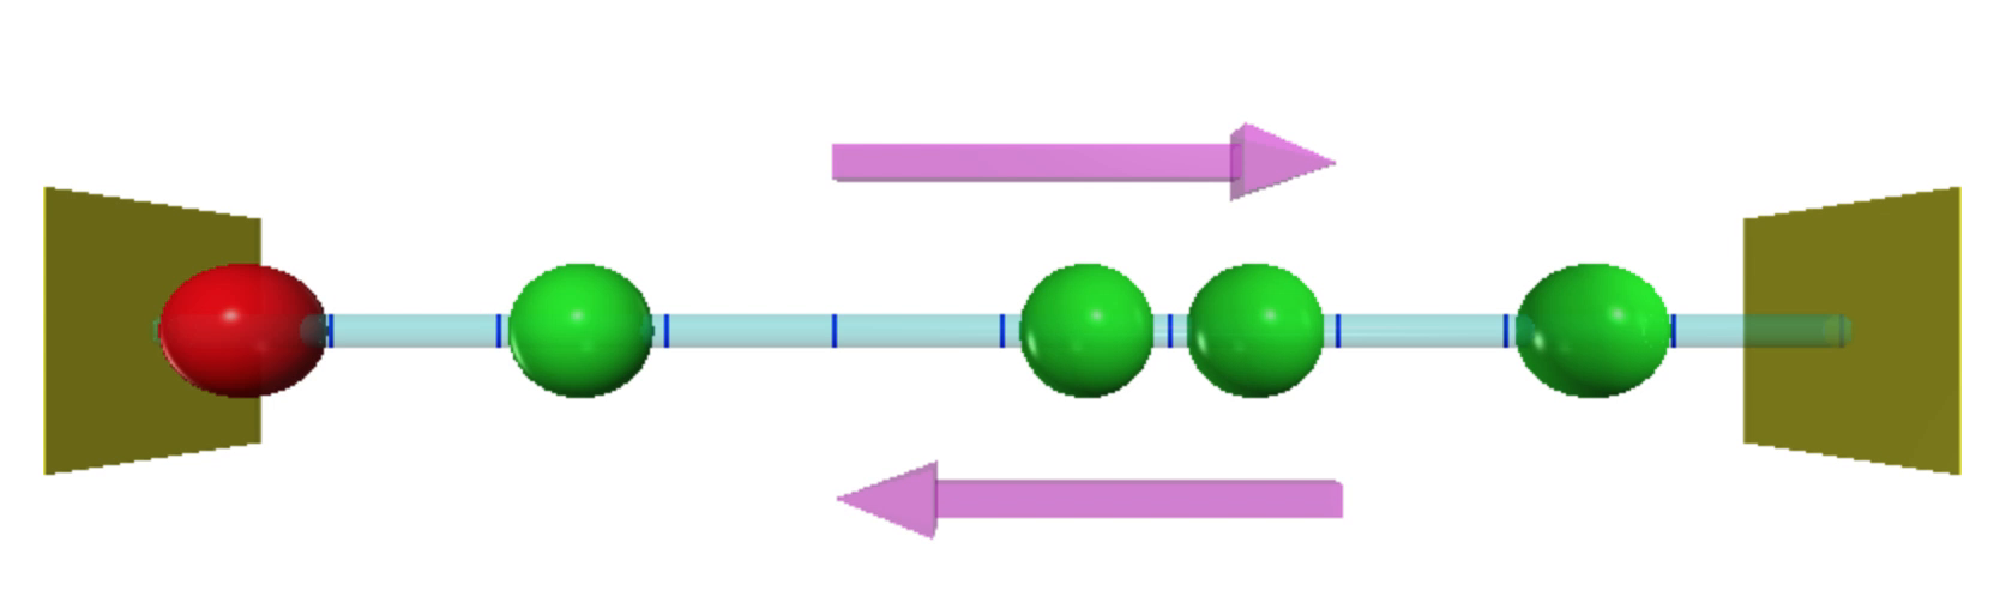
\includegraphics[width=0.8\linewidth]{betheEq}
    \caption{Intepretation of Bethe Equation.}
    \label{fig:betheEq}
\end{figure}
By solving the Bethe equation, one can get $p_1$ and $p_2$ and thus all
amplitude coefficients up to a constant normalization factor. Then Eq.
\eqref{eq:eigenvaluesTwo2} gives the eigenvalues and Eq.
\eqref{eq:nonstationaryModesTwo2} gives the eigenfunctions.
Unfortunately, it might not possible to solve the Bethe equation analytically.
So we resort to numerical solutions. We have verified the resulting eigenvalues
and eigenfunctions by benchmark with the results from brute force diagonalizing
of the transition matrix for small system size $L\le10$. Notice that those roots
that $p_n=0$ or $p_n=\pi$ have to be filtered out because they correspond to the
first type of non-stationary eigenmodes which is not compatible by Eq.
\eqref{eq:nonstationaryModesTwo2}


To summarize, the complete solution of two particle hopping system with
reflecting boundaries was found. The solution is shown in the form of
eigenfunction expansion, i.e. Eq. \eqref{eq:eigenModesTwo}. The stationary
eigenfunction with eigenvalue $\Lambda_0=0$ is listed as Eq.
\eqref{eq:stationaryTwo}, while the two types of non-stationary eigenvalues and
corresponding eigenfunctions are listed in Eq. \eqref{eq:eigenvaluesTwo1},
\eqref{eq:eigenvaluesTwo2} and Eq.
\eqref{eq:nonstationaryModesTwo1}, \eqref{eq:nonstationaryModesTwo2},
respectively. They can be fully determined by  solving the Bethe Equation Eq.
\eqref{eq:betheEqTwo1} and Eq. \eqref{eq:betheEqTwo2}. Part of them are
analytically shown in Eq. \eqref{eq:eigenTwo}.

Finally, there are several remarks we want to make here.
Firstly, as one can see from Eq.  \eqref{eq:eigenTwo} that the eigenvalues of two
particle system always contain the eigenvalues of single partile system. We will
show later this can be generalised that the eigenvalues of $N+1$ particle system
always contain the eigenvalues of $N$ particle system for $N<L/2$. Secondly, the
relaxation time of the system is realted to the largest non-zero eigenvalue
$\Lambda_1$. Eq.  \eqref{eq:eigenTwo} hints
$\Lambda_1=-(\alpha+\beta)+2\sqrt{\alpha\beta} \cos\left(\frac{\pi}{L}\right)$.
However, since there is no analytical solution for eigenvalues of the second
kind, it will be difficult to rigously prove that. Nummerical evidences will be
provided to verify this is indeed true.

In next section, we will generalise the solution to the $N$ particles system.
It is actually quite straight forward after we have done the two particles
case. 


\section{General Solution of $N$ particles ASEP}
\label{sec:general_solution_of_n_particles_asep}

As before, we first write down the master equation of a $N$ particles system.
\begin{equation}
    \begin{aligned}
        \label{eq:masterEqN}
        \frac{d P(x_1, \cdots, x_N; t)}{dt} = & \sum_{j=1}^N \left[\alpha
            P(\cdots,x_j-1,\cdots;t) + \beta P(\cdots, x_j+1, \cdots;t)\right. \\ 
        & \left.- (\alpha+\beta)P(\cdots, x_j, \cdots; t)\right]
    \end{aligned}
\end{equation}

Similarly, after the eigenfunction expansion the reflecting boundaries write as
\begin{subequations}
    \label{eq:boundaries-N-particles}
    \begin{eqnarray}
        \alpha \Psi(0,x_2,\cdots,x_N) = \beta \Psi(1, x_2,\cdots, x_N) \\
        \alpha \Psi(x_1,\cdots, x_{N-1}, L) = \beta \Psi(x_1,\cdots, x_{N-1}, L+1)
    \end{eqnarray}
\end{subequations}
The exclusive condition for $N$ particles case is more tricky. In principle,
one has to consider to case of three body collision and four body collision and
so on. Luckily, in the simple model of ASEP, one can prove that these more than
two body exclusive conditions are not new but just linear recombination of two
body exclusive condition. So we can write the exclusive condition of a $N$
particles system as 
\begin{equation}
    \label{eq:exclusionConditionN}
    \alpha \Psi(\cdots,x, x,\cdots) + \beta \Psi(\cdots, x+1, x+1, \cdots) 
    = (\alpha + \beta) \Psi(\cdots, x, x+1, \cdots)
\end{equation}
The reason that the exclusive condition can be written in such a simple way is
rooting from the Yang-Baxter Equation, which encodes the integrability of the
ASEP system.

\subsection{Stationary Solution}
\label{sub:stationary_solution}

Intuitively, we construct the $N$ particles stationary solution as
\begin{equation}
    \label{eq:stationaryN}
    P^e(x_1, x_2, \cdots, x_N) = \Psi(x_1, x_2, \cdots, x_N) =  A
    \prod_{j=1}^N\left(\frac{\alpha}{\beta}\right)^{x_j}
\end{equation}

One can plug in the master equation check that the corresponding eigenvalue
$\Lambda_0= 0$, and also verify the exclusive condition as well as the reflecting
boundaries are fulfilled by insert the solution in to Eq.
\eqref{eq:exclusionConditionN} and Eq. \eqref{eq:boundaries-N-particles}
separately.

We now try to fix the parameter $A$ by normalization. Let us denote
$q:=\frac{\alpha}{\beta}$, then we can write $A$ as following
\begin{equation}
    \label{eq:stationaryPrefactor}
    A^{-1} = \sum_{\Omega} q^{\sum_j{x_j}} = 
    \sum_{x_1 < x_2 < \cdots < x_N} q^{\sum_j{x_j}}
\end{equation}
Let us do a variable change so that 
\begin{eqnarray*}
    \sum_j{x_j} &=& E_0 + E \\
    E_0 &=& 1 + 2 + \cdots + N = \frac{N(N+1)}{2}
\end{eqnarray*}
We can derive that $E$ is a integer in the range of $0, 1, \cdots, N(L-N)$. So
Eq. \eqref{eq:stationaryPrefactor} can be rewrite as 
\begin{equation}
    \label{eq:prefactorRewrite}
    A^{-1} = q^{E_0}\sum_{E=0}^{N(L-N)}g(E)q^E
\end{equation}
where $g(E)$ is the number of partitions of positive integer $E$ to $N$ parts
with each of size at most $L-N$. From the number partition theory, we identify
\begin{equation}
    \label{eq:degeneratcy}
    \sum_{E=0}^{N(L-N)}g(E)q^E = \binom{L}{N}_q =
    \frac{[L]_q!}{[L-N]_q![N]_q!}
\end{equation}
where $[N]_q = 1 + q + q^2 + \cdots + q^{N-1}$ is called a $q$ number, and Eq.
\eqref{eq:degeneratcy} is called the $q$ binomial coefficient\cite{}.
So we finally arrive at 
\begin{equation}
    \label{eq:stationarySolutionN}
    P^e(x_1, x_2, \cdots, x_N) = q^{-\frac{N(N+1)}{2}}
    \binom{L}{N}_q^{-1}\prod_{j=1}^N{q^{x_j}}
\end{equation}

In \cite{}, G. M. Sch\"{u}tz use a quantum group formalism obtained the same
result with a different notation. We emphasize here that our method is much more
easily to understand and no prerequisite knowledge of quantum mechanics and
group theory is needed.

With the equilibrium $N$ particle distribution, we can readily calculate the
equilibrium distribution of any tagged particle. Denote he distribution of the
$n$th particle $p_n(x)$, we have
\begin{equation}
    \begin{aligned}
        \label{eq:pdfTaggedParticle}
        p_n(x) = & \sum_{0<x_1<\cdots<x_{n-1}\le x-1}P^e(x_1, x_2, \cdots, x_N)
        \sum_{x<x_{n+1}<\cdots<x_{N}\le L}P^e(x_1, x_2, \cdots, x_N) \\
        = & \left. q^{(N+1-n)(x-n)} \binom{x-1}{n-1}_q\binom{L-x}{N-n}_q 
            \middle/  \binom{L}{N}_q \right.
    \end{aligned}
\end{equation}
Finally, the equilibrium density profile can be obtain by summing up $p_n(x)$
\begin{equation}
    \label{eq:densityProfile}
    \rho(x) = \sum_{n=1}^N p_n(x) 
\end{equation}


\subsection{Non-stationary Modes}
\label{sub:non_stationary_modes}

Inspired by the calculation of two particles case, we try to find the Bethe
solution of the $N$ particles system by taking the following Ansatz: 
\begin{equation}
    \label{eq:nonstationaryModesN}
    \begin{aligned}
        \Psi(x_1, x_2, \cdots, x_N) = \sum_{\sigma\in \mathcal{S}_N}
        \prod_{n=1}^N \psi_n^{\sigma}(x_{\sigma(n)})
    \end{aligned}
\end{equation}
where $\mathcal{S}_N$ is the group of permutations of $N$ elements and
$\psi_n^{\sigma}$ is the $n^{\text{th}}$ class of eigenfunction of Eq.
\eqref{eq:eigenModes}, either stationary or non-stationary. The subscript $n$
means all functions in the $n^{\text{th}}$ class share the same $p_n$, the
superscript $\sigma$ means the amplitude coefficients $A_n^{\sigma}$ or
$A_{n\pm}^{\sigma}$ are not the same for different permutations.

We again insert the solution to the master equation Eq. \eqref{eq:masterEqN},
notice that the amplitude coefficients are irrelevant with the eigenvalues. So
we obtain the simple form of corresponding eigenvalue 
\begin{equation}
    \label{eq:eigenvaluesN}
    \Lambda = \sum_{n=1}^N \lambda_n
\end{equation}
$\lambda_n$ here is a function and its expression depends on whether
$\psi_n^{\sigma}$ is stationary or non-stationary. For stationary $\lambda_n=0$,
for non-stationary $\lambda_n(p_n)=
-(\alpha+\beta)+2\sqrt{\alpha\beta}\cos(p_n)$.  Notice that, as we can see from
the two particles example, the Bethe Equations will give the value of $p_n$ and
determine the eigenvalues. In general, they are more than one solution because
Bethe Equations are nonlinear, and different solution can lead to different
eigenvalues.

We now consider that the non-stationary eigenfunctions is constructed by $N_s$ of
Eq. \eqref{eq:stationaryEigenMode} classes and $N-N_s$ of Eq.
\eqref{eq:nonstationaryEigenModes} classes. Notice that $N_s=0$ corresponds to
the second type of eigenfunctions in our discussion of the two particles system.
We will start from this case first here.

Plug Eq. \eqref{eq:nonstationaryModesN} in to the reflecting boundaries Eq.
\eqref{eq:boundaries-N-particles} we can obtain 
\begin{subequations}
    \label{eq:scatterFactorBoundaryN}
    \begin{eqnarray}
        \frac{A_{n+}^{\sigma|\sigma(1)=n}}{A_{n-}^{\sigma|\sigma(1)=n}} & = &
        -\frac{\alpha-\sqrt{\alpha\beta}
            e^{-ip_{n}}}{\alpha-\sqrt{\alpha\beta} e^{ip_{n}}}
        \\ \frac{A_{n+}^{\sigma|\sigma(N)=n}}{A_{n-}^{\sigma|\sigma(N)=n}} & = &
        -\frac{\left(\alpha-\sqrt{\alpha\beta} e^{-ip_{n}}\right)
            e^{-ip_{n}L}}{\left(\alpha-\sqrt{\alpha\beta}
                e^{ip_{n}}\right) e^{ip_{n}L}}
    \end{eqnarray}
\end{subequations}
And substitute the Ansatz in to the Exclusive condition Eq.
\eqref{eq:exclusionConditionN} we get
\begin{subequations}
    \label{eq:scatterFactorExclusiveN}
    \begin{eqnarray}
        \frac{A_{n\pm}^{\sigma}A_{(n+1)\pm}^{\sigma}}{A_{n\pm}^{\sigma|
                n\leftrightarrow n+1}A_{(n+1)\pm}^{\sigma|n\leftrightarrow n+1}}
        & = & -\frac{a(\pm p_{n},\pm p_{n+1})}{a(\pm p_{n+1}, \pm p_{n})} \\
        a(p, p^{\prime}) & = & \sqrt{\alpha\beta}e^{i(p+p^{\prime})} - (\alpha +
        \beta) e^{i p} + \sqrt{\alpha\beta}
    \end{eqnarray}
\end{subequations}
% \begin{equation}
%     \label{eq:consistencyConditionN}
%     \frac{A_{n+}^{\sigma|\sigma(1)=n}}{A_{n-}^{\sigma|\sigma(1)=n}}  
%     \frac{A_{n-}^{\sigma|\sigma(N)=n}}{A_{n+}^{\sigma|\sigma(N)=n}} = 
%     \frac{\tilde{A}_{1}\tilde{A}_{2+}}{A_{1}A_{2+}}
%     \frac{A_{1}A_{2-}}{\tilde{A}_{1}\tilde{A}_{2-}}
% \end{equation}
Then one can either use the consistency condition or the interpretation we
discussed in the two particles case and the well know periodic Bethe Equation,
easily find the following set of Bethe Equations for the $N$ particles system:
\begin{equation}
    \label{eq:betheEqN}
    e^{i2p_nL}  =  \prod_{m\neq n}^N\frac{a(p_n, p_m)}{a(p_m, p_n)} 
    \frac{a(p_m, -p_n)}{a(-p_n, p_m)}
\end{equation}
By solving Eq. \eqref{eq:betheEqN} we get all the $p_n$ and then one can plug
back in Eq. \eqref{eq:eigenvaluesN} and Eq. \eqref{eq:nonstationaryModesN} for
the corresponding eigenvalues and eigenfunctions. 

Now let us come back to the case that $0<N_s<N$. The calculation of the two
particles system is a good illustration. We can easily find out there is
nothing different except we will have only $N-N_s$ wave vectors and $2N-N_s$
amplitude coefficients. So one just have to use the relation similar to Eq.
\eqref{eq:scatterFactorExclusive} together with Eq.
\eqref{eq:scatterFactorBoundaryN} to build the Bethe Equation. Moreover, Eq.
\eqref{eq:betheEqTwo1} tells us that the Bethe Equations we can obtain will be
exact the same as the Bethe Equations of the second type $N-N_s$ particles
system. So according to Eq. \eqref{eq:eigenvaluesN} for the eigenvalues, we can
conclude that the eigenvalues of $N-N_s$ particles system are always contained
in the eigenvalue set of $N$ particle system. Notice that this is only true for
$N<L/2$. For $N>L/2$, one can easily use the particle-hole duality which shows
that the eigenvalue of $N$ particles system should be the same as $L-N$
particles system.
\begin{figure}[htpb]
    \centering
    \includegraphics[width=0.8\linewidth]{spectrum}
    \caption{Left: embeding of eigenvalues; Right: benchmark of eigenvalues from
        Bethe Ansatz theory to directly diagonalize transition matrix, $N=2$.
        $L=10$, $\alpha=2$ and $\beta=1$ for both. }
    \label{fig:spectrum}
\end{figure}

Finally, we remark that the Bethe Equations have to be solved numerically in
most cases. However, there is a small set of non-stationary eigenvalue and
eigenvectors we can obtain analytically, which correspond to the case with
just one excitation mode. The results are summarized as following:  
\begin{subequations}
    \label{eq:eigenN}
    \begin{eqnarray}
        \label{eq:partEigenvaluesN}
        \Lambda_k  = 
        -(\alpha+\beta) + 2\sqrt{\alpha\beta}\cos(\frac{k\pi}{L});
        ~k=1,2,\dots, L-1  \\
        \label{eq:eigenvectorsN}
        \Psi_k(x_1, x_2, \cdots, x_N)  =  A \sum_{n=1}^N
        \left(\frac{\alpha}{\beta}\right)^{n-1} \phi_k(x_n)\prod_{m\neq n} 
         \left(\frac{\alpha}{\beta}\right)^{x_m}
    \end{eqnarray}
\end{subequations}
Notice that the set of eigenvalue is exact the single particle spectrum, and
again $\phi_k(x)$ is exactly the single particle eigenfunction.
Fortunately, the numerical evidence shows that the most interesting
eigenmode, i.e. the slowest relaxation mode, is contained in this set. 
We will discuss it in next section. 

\section{Relaxation Time}
\label{sec:relaxation_time}

The largest non-zero eigenvalue we found and verified by numerical results is 
\begin{equation}
    \label{eq:largestEigenvalue}
    \Lambda_1 = -(\alpha+\beta) +
    2\sqrt{\alpha\beta}\cos(\frac{\pi}{L})
\end{equation}
If $L \gg 1$, we can expand the cos term, obtain 
\begin{equation}
    \label{eq:largestEigenvalueExpanded}
    \Lambda_1 = -(\sqrt{\beta}-\sqrt{\alpha})^2 -
    \frac{\sqrt{\alpha\beta}\pi^2}{L^2}
\end{equation}
And the relaxation time can be calculated as 
\begin{equation}
    \label{eq:relaxationTime}
    \tau = -\frac{1}{\Lambda_1}
\end{equation}

There are several information we can read form Eq.
\eqref{eq:largestEigenvalueExpanded} and \eqref{eq:relaxationTime}. Firstly, we
can see the scaling $\tau \approx L^2$, which means the dynamical exponent of
the system is $2$. Secondly, as we can see from Eq.
\eqref{eq:largestEigenvalueExpanded}, the bigger difference between $\alpha$
and $\beta$, the smaller relaxation time we will get. This is also consistent
as one would expect. If we map back to the polymer model, the result here can
be compared with the prediction of Rouse theory. Unlike the prediction
from Rouse theory that relaxation time does not depend on external force, we
have here that stronger external force decreases the relaxation time. This
point highlight the fundamental difference between the infinite extensible bead
spring model and the rigid bead rod model which is of course finite extensible. 

In Fig.  \ref{fig:eigenvalues} shows all the eigenvalues of a system with
lattice size $L=10$, calculated by brute force diagonalizing the transition
matrix.  Lattice The number of particles on the lattice is ranging from $1$ to
$9$. The difficult to calculate larger lattice size $L$ lies on that the
dimension grow as $\binom{L}{N}$, and if we take $N=L/2$, the dimension of the
matrix will became a extremely large number very soon. 

\begin{figure}[htpb]
    \centering
    \includegraphics[width=0.8\linewidth]{eigenvalues}
    \caption{Eigenvalues calculated by numerically diagonalize the transition
        matrix.}
    \label{fig:eigenvalues}
\end{figure}

As we can see in Fig. \ref{fig:eigenvalues}
that all eigenvalues of case $N=1$ are contained in the set of
eigenvalues $N=2$, and all eigenvalues of case $N=2$ are contained in the set
of $N=3$ and so on until reach the largest set $N=L/2$. This means the
characteristic polynomial of $N=k+1$ always contains the factor of the
characteristic polynomial $N=k$. This is predict exactly by our theory. 

\section{Summary}
\label{sec:summeary}
We use the modified Bethe Ansatz methods solve the ASEP model with reflecting
boundaries.  The stationary distribution was solved exactly and the one
correspond to the relaxation time of the system was postulated. Numerical
evidence is provided for later statement.

\newpage

\appendix
\section{Derivation of the exclusion condition}
To derivate the exclusion condition, which is a little bit confusing at a first sight, we use the two particles example and then generalise to $N$ particle case.
First, let us rewrite the master equation of this two particle system:
\begin{equation}
    \begin{aligned}
        \label{eq:masterEqTwoGeneral}
    \frac{d P(x_1, x_2; t)}{dt} = & \alpha P(x_1-1,x_2;t) + \beta P(x_1+1,x_2;t) \\ 
    & + \alpha P(x_1, x_2-1; t) + \beta P(x_1, x_2+1; t)  \\ 
    & - 2(\alpha+\beta)P(x_1, x_2; t)
    \end{aligned}
\end{equation}
We assume the above equation is valid for the whole space. However, this is actually not true when the two particles are sitting on the neighboring sites. Let us now consider this special case separately, remember that $x_2 = x_1 + 1$. The master equation of this special case can be written as
\begin{equation}
    \begin{aligned}
        \label{eq:masterEqTwoNeighbor}
        \frac{d P(x_1, x_2; t)}{dt} = 
        & \alpha P(x_1-1,x_2;t) + \beta P(x_1, x_2+1; t)  \\ 
    & - (\alpha+\beta)P(x_1, x_2; t)
    \end{aligned}
\end{equation}
Now, let us do a subtraction, i.e. \eqref{eq:masterEqTwoGeneral} $-$ \eqref{eq:masterEqTwoNeighbor}, obtain
\begin{equation}
    \alpha P(x_1, x_2-1; t) + \beta P(x_1 + 1, x_2; t) = (\alpha + \beta)P(x_1, x_2; t)
\end{equation}
Let us then denote $x:=x_1$ and plug in $x_2 = x_1+1 = x+1$ in the above equation. We finally arrive at
\begin{equation}
    \label{eq:exclusionConditionTwo}
    \alpha P(x, x; t) + \beta P(x+1, x+1; t) = (\alpha + \beta)P(x, x+1; t)
\end{equation}

In summary, the sole master equation Eq. \eqref{eq:masterEqTwoGeneral} does not take into account the exclusion cases. In order to represent the exclusive setting, we assume Eq. \eqref{eq:masterEqTwoGeneral} is valid for the whole space, and then apply an additional condition on this equation like Eq. \eqref{eq:exclusionConditionTwo}. This condition is similar to the partial derivative of the PDF is the same at the collision boundary $x_1 = x_2$ in the continuous space case. 

Finally, in the similar way we can derive the exclusion condition for the cases $N>2$. However, it is not difficult to check that in cases of more than two particles, the three body collision or four body collision cases do not give out new conditions, just the linear combination of the two body collision conditions like Eq. \eqref{eq:exclusionConditionTwo}. This is fundamentally a result of Yang-Baxter Equation is satisfied for the ASEP model.

% \bibliography{report}
\bibliographystyle{plain} 

\end{document}
